\chapter{Omniscient Debugging Across System Boundaries}
\label{sec:stack_odb}


%\section{A System-independent View on Debugging}
%
%\section{Detecting Inter-System Program Flow}

\tmpStart

% Context: architectures
Complex applications are rarely single programs running on a single machine but often consist of multiple components implemented in different programming languages and running in different environments.
A notable example is the multi-tier architecture, a successful and established pattern for client-server applications since over two decades.

% Problem
Breaking down applications into layers and sub-systems allows for better scalability and easier life-cycle management, but makes debugging such applications much harder.
Software failures are typically observed in the front-end first.
Then, developers have to guess which layer contains the fault. 
Otherwise, they have to switch debugging tools frequently while they track the infection chain across the entire software stack.

% Signifiance
In the past, this problem was mitigated because most application code resided in the business tier, while the presentation and data tiers only served to display back-end provided views and to persist application state, respectively.
However, changes in technologies and requirements caused more code to move up or down the stack, thereby increasing the need to debug the application as a whole.
Service-oriented architecture and micro-services are more recent patterns that exacerbate the problem by dividing applications into even more independent components.

% Solution
We interviewed software developers on the difficulties when developing modern enterprise applications.
Based on these insights, we developed a prototype for a back-in-time debugger allowing developers to debug the full stack of a 3-tier application in one session.

Assuming back-in-time debugging capabilities for each application tier, we introduce hierarchical step numbering based on synchronization points between components to create a partial ordering of instructions in all concurrent executions.
A visualization shows which UI element is affected by which back-end operation, providing developers with a top-down summary of the execution.
A second visualization is shown in the debugger and helps developers to navigate the application flow.


Based on the collected developer experience, we built a back-in-time debugger for 3-tier applications running in SAP HANA.
We then collected developer feedback for our prototype.
Based on this feedback, we identified suggestions how existing debugging tools can be improved even without the need for resource-intensive back-in-time debugging.

%The remainder of this paper is structured as follows:
%The next section summarizes related work.
%\Cref{sec:interviews} discusses the results of our interviews. 
%We describe in more detail how 3-tier applications have changed in the last decade and which information developers need when debugging such applications.
%\Cref{sec:debugger} presents our prototype implementation of a full-stack back-in-time debugger.
%\Cref{sec:conclusion} concludes.
%
%\section{A Prototype for Full-stack Back-in-time Debugging}
%\label{sec:debugger}

%We tested the debugger on the POS explorer and were able to seamlessly debug the entire application stack, while providing additional high-level visualizations

\section{Obtaining the Full Execution History}

For the purpose of our debugger, we assume that omniscient debugging capabilities for each layer already exist.
This means that we need not only the ability to move execution forwards and backwards, but also a way to search the entire history for specific instructions.
At the very least, we need a way to obtain full traces of all layers that we can store in a database.

In this context, we call an \emph{execution} the invocation of a function or method in a layer that was triggered by an external event, such as a request or a response from a different layer, and that is traced independently of other previous, concurrent, or future executions.
The \emph{full execution history} is the set of all executions that were transitively caused by a root execution.
In the full history, multiple executions that may appear to be independent are grouped together as they are part of the same higher-level operation.

To be able to fully restore the program state from any point in time, traces need to contain not only all method invocations, but also all variable assignments and all field accesses.
For the technologies involved, no tracing tools that could provide the required level of detail existed at the time.

For the data layer, we used our existing omniscient debugger for stored procedures.%~\cite{treffer2017bringing}.
It inserts trace statements into the code that save the execution in the database.

In the application layer, the server runtime needs to collect and store the trace.
Since the SAP HANA platform has no such capabilities at this time, we used a similar approach as with the stored procedures debugger.
A pre-processor parses the JavaScript files and inserts trace statements for all instructions.
Then, to collect a trace, the actual back-end code has to be temporarily replaced with the modified tracing code.

In the front-end, the browser or a browser plug-in can be used to collect the execution trace.
However, while there exist many tracing plug-ins for all modern browsers, most are designed for performance profiling and therefore don't provide the necessary level of detail.
We also found that many browsers provide a debugging interface that could be used to implement a tracing plug-in.
Nevertheless, for now we again used our JavaScript pre-processor.
For simplicity, we only traced the application code and not the SAPUI5 and jQuery libraries.

Both the front-end and the back-end JavaScript tracer first store the entire trace in an array and then, at the end of the execution, submit it to the database.
From the front-end, data is sent via an HTTP POST request and then passed on to the database via a back-end script.
All JavaScript execution traces are stored in a single relational database schema, the execution traces of stored procedures are stored in a second, slightly different schema.

In the POS explorer, drop-down boxes allow to select filter criteria that are then applied to all components on the dashboard.
\Cref{fig:pos} on page~\pageref{fig:pos} shows a section of the user interface.
The green and red boxes were inserted by our debugger and can be ignored for now.
Selecting, for example, "BACONSNACKS" from the category drop down at the top of the screen updates five UI components of which three are shown in \cref{fig:pos}.

In total, this operation generates almost 400 traced instruction in the back-end, libraries excluded.
Due to the asynchronous nature of AJAX requests, those events are split over 5 separate executions.
Four HTTP requests to the back-end create four executions with around 800 traced instructions each.
Each back-end request triggers one stored procedure, each with 17 to 25 traced instructions.

\section{Identifying Sub-system Interactions}

When all operations have completed, we have traced a total of 13 executions.
To allow seamless debugging of the entire application, we now have to restore the request/response relations that define the application flow.
Since most requests are handled concurrently, we can not simply use timestamps to recreate the order.

In a first step, we select all executions from the trace databases that occurred in the time-frame of the front-end operation and number them in order of the time stamp of the first recorded instruction.
Then we create a mapping between execution number and its schema and the execution id within that schema.
This mapping will later be needed for uniquely identifying each point in time while allowing for sequentialized debugging of concurrent executions.

In the second step, we collect all requests that were sent from each layer.
This step is technology-specific.
For the front-end, we scan the trace database for invocations of ´jQuery.ajax()´ and determine the request URL to later identify the request.
In the application layer we scan for invocations of ´execute()´ on prepared-statement objects and determine the query string.

In both cases, our prototype was specifically tailored for the POS explorer.
First, there are many different ways in which a request can be sent and we covered only the ways that were actually used.
Second, when determining the URL and query strings we took advantage of the fact that the strings were always stored in a variable of the same name.
For a generalized solution, the debugger needs to perform a small dynamic code analysis to identify the correct values.
With full access to the code and the execution trace, this analysis should not be too difficult to perform, but for now it was beyond the scope of our project.

In the third step, we determine for each execution by which request it was triggered.
In the application layer, we inserted special tracing code to record the request URL, which then only has to be matched against the URLs requested by the front-end.
To match stored procedure calls, we check which query string contains the procedure name as a sub-string.
Finally, four executions in the front-end were triggered by asynchronous AJAX results.
Here, we used the fact that the response is handled in the same file from which the request was sent to find the original request.

In the case of the POS explorer, this was enough to unambiguously match all request and response relations.
In other scenarios, where multiple very similar requests are sent, other approaches may be needed.
For example, unique arguments could be added to request URLs to allow for better matching of executions.
In the case of database requests, the runtime environment probably has better ways of matching requests, such as internal connection ids.
With a better integration of tracing in the platform, such data can be easily recorded and used accordingly.

\section{High-level Visualizations}

% component11
% component13
% component14
% component15

All developers we interviewed reported that they prefer to begin debugging by understanding the high-level interactions first.
Now that the debugger can successfully identify these interactions, they can be visualized in the user interface.
Our prototype provides two visualizations.

First, calls to the back-end layers are shown directly on the web page, right next to each UI component, as shown in~\cref{fig:pos}.
This allows developers to immediately see which request belongs to which component, which is particularly helpful if only one component shows incorrect data.

\begin{figure}
	\centering
		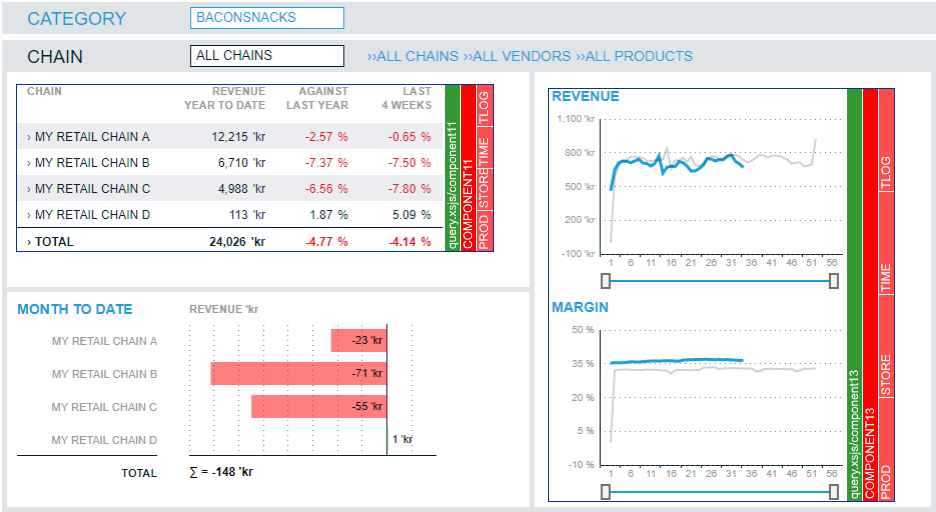
\includegraphics[width=1.00\linewidth]{img/pos.png}
	\caption{A section of a KPI dashboard. Directly next to UI components, elements were inserted that show which back-end functions and data sources provided the displayed data.}
	\label{fig:pos}
\end{figure}

In our prototype, mapping requests to UI components is possible because we can track from which component's ´refresh()´ method the request was sent.
As can be seen, the bar chart at the bottom left has no associated requests shown because it reuses data from the table above.
For a more generalized solution, code analysis can be used to determine to which UI components data is passed.
This will work even for scenarios where a central refresh method updates all components or where client-side post-processing of the data is performed.

Colors are used to show the involved application layers.
The green box shows the path of the request URL, the red boxes show the names of the stored procedures and database tables that where subsequently accessed.

Second, the debugger window, as shown in~\cref{fig:debugger}, shows a full overview of all interactions.
The largest part of the debugger windows is occupied by the source code.
To the right, current variable values are shown.
At the top of window, a diagram shows the entire history of all individual executions and their request/response relations.

\begin{figure}
	\centering
		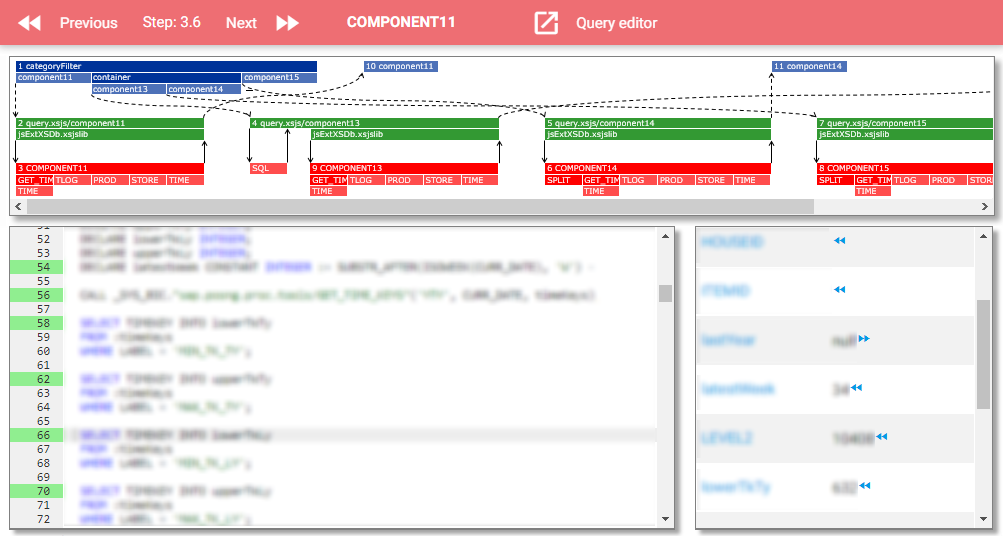
\includegraphics[width=1.00\linewidth]{img/debugger_full.png}
	\caption{A screenshot of our debugger prototype. On top of the code and variables view, a diagram shows the flow of requests in the application.}
	\label{fig:debugger}
\end{figure}

\begin{figure}
	\centering
		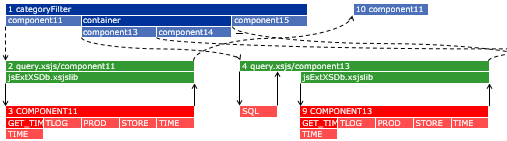
\includegraphics[width=1.00\linewidth]{img/executions.png}
	\caption{A part of the interaction diagram. Colors encode the application layer, dashed arrows represent asynchronous, solid arrows represent synchronous requests and responses.}
	\label{fig:executions}
\end{figure}

\Cref{fig:executions} shows a part of the interaction diagram in more detail, with anonymized names.
Each group of adjacent rectangles represents one execution trace.
The execution number and name are shown in the topmost rectangle of each group.

For the front-end, shown in blue, the blocks represent the hierarchy of UI components.
In the application layer, green blocks show the files that were executed to respond to requests and below files that submitted database queries.
Red blocks, finally, show the stored procedures that were called and, in lighter red, the tables that were accessed.
At the beginning of execution \#4 in the application layer, a plain SQL query is submitted to the database, not calling any procedures.

The length of the rectangles has no significance, in particular it does not reflect execution times.
Between the layers, asynchronous calls are shown with dashed lines, synchronous calls with solid lines.

The diagram is interactive.
For example, clicking the arrows reveals details about the requests.
For HTTP requests, the request URL and arguments and the response body are shown.
Clicking a database request opens a query window with the query string.
This allows developers to inspect the query result and to modify the query, which can help to better understand the data.
Finally, clicking a rectangle moves the debugger to the point in time where the respective code is executed.

\section{Debugging the Full Stack}

After developers have gained an overview over the full execution history and maybe formed first hypotheses about the bug, they want to begin debugging the code.
With the entire execution history recorded, a post-mortem debugger can replay the execution.

To identify a point in time, the debugger needs the execution number and the instruction index within the execution.
From the execution number, the debugger resolves which trace database to use.
Then, with the instruction index the current code location and program state is restored.
Stepping forwards and backwards changes the instruction index within the execution.

Typically, a back-in-time debugger allows to step forwards and backwards within a method and into and out of method calls.
When an instruction is reached that is associated with a request to another layer, 
an additional option is given to step into the execution that handles the request.
For asynchronous requests, developers can also directly jump to the execution that handles the response.
Within any request-handling execution, stepping out of the root method call moves the debug session to the instruction where the response is received.

When a higher layer sends a request down the software stack, the debugger has to decide at which point to move to the request-handling execution.
For example, developers typically don't want to debug jQuery internals or the database driver when searching a bug in the application code.
The situation becomes more complicated when the application uses a custom abstraction layer on top of the library that is used to actually send the request.
This abstraction needs to remain debuggable, because it may contain bugs, but we also want to avoid slowing down developers every time they want to follow a request.

Our debugger prototype allows developers to store a custom list of request commands, which are specified using a sub-set of XPath.
For example, a developer might specify "´//sendSQL´" to mark a method that builds and submits an SQL query string.
All method invocations that match the XPath pattern will be associated with a request, if a request was sent from within that invocation, no matter how deeply nested.
When the developer reaches such an invocation in the debugger or debugs within such an invocation, the buttons for jumping to the request and to the response handler are shown.

In our prototype, the XPath expression can contain only node names that are matched against method names, using only the child and descendants axes.
However, additional axes and predicates (e.g., to filter for methods of a certain class) could be implemented with our approach.

On top of the simplified navigation of the application stack, additional synergy effects can occur when integrating the debuggers.
Our omniscient debugger for stored procedures allows to query the database from previous points in time.%~\cite{treffer2017bringing}.
An extension to SQL allows developers to specify steps from the execution of the stored procedure in their queries.
We enabled the back-in-time query feature for all layers.

Developers can use hierarchical step numbers, e.g. "1.17" for the 17th step of the first execution, to select points in time in SQL queries.
A query pre-processors maps this number to a database snapshot.
If the execution number does not represent a stored procedure, the next stored procedure call is looked up by following requests from the application flow graph and the first step of that execution is used as a point-in-time.
If there is no next stored procedure call, the last step of the last previous call is used.
After that, the stored procedure steps are converted into timestamps using the mechanisms that are already in place.

Allowing to query the database from all layers has two advantages.
First, developers can look at the data while debugging the front-end.
No switching of tools is required and the database is automatically shown as it was at the respective point in time.
Second, developers can now query for changes in the data that happens across multiple executions.
For example, \cref{lst:tdiff} shows a back-in-time query that selects all products whose margin-attribute changed between the beginning of the first execution (step~1.1) and the beginning of the first response handler (step~10.1, cf.~\cref{fig:executions}).

\begin{lstlisting}[language=HanaSQL,float=t,caption={A query selecting all products whose margin was changed during the operation.},label=lst:tdiff,numbers=none]
	SELECT p.name, p.margin
	FROM Products p
  WHERE ^start!^p.margin != ^now!^p.margin
	^§AT STEP§ start=1.1, now=10.1^
\end{lstlisting}

%todo: synergy

\section{Developer Feedback}

We showed our debugger prototype to the developers we initially interviewed to understand the development and debugging processes in 3-tier business applications.

All developers immediately liked the idea of displaying back-end operations directly in the user interface.
Such a feature would not only be useful for debugging, but also for documentation purposes.
The developers also wished that this visualization was interactive like the interaction diagram, i.e., that clicking the boxed showed details about the requests and allowed to jump to the respective instruction in the debugger.
One developer argued that showing the back-end operations in a three dimensional stack would allow to show more details, especially in user interfaces with smaller individual components.
\Cref{fig:3d} shows a mock-up of the idea.

\begin{figure}
	\centering
		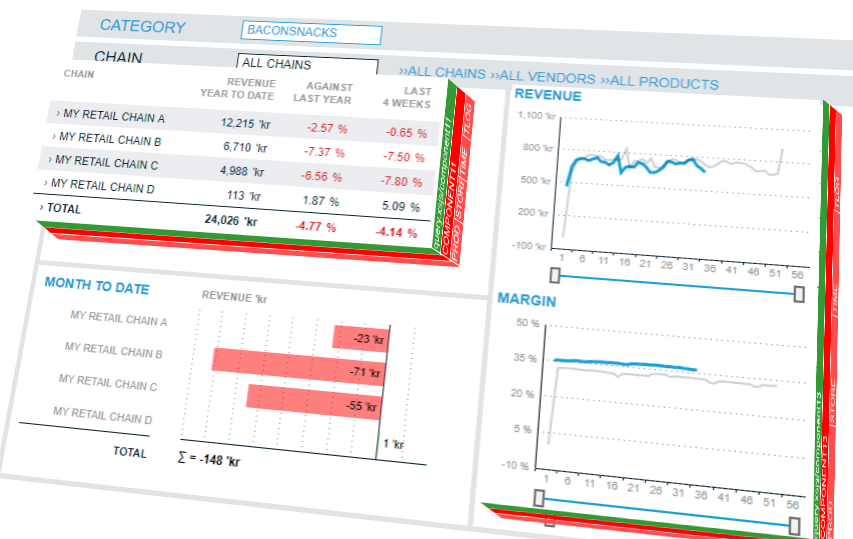
\includegraphics[width=1.00\linewidth]{img/pos3d.png}
	\caption{3D visualization of the software stack in the front-end. Developers can tilt the page to read debugging information on the side of the stacks.}
	\label{fig:3d}
\end{figure}

The interaction diagram was perceived as equally useful.
The developers generally liked the idea of not arranging elements based on timing related information, which allows for a clearer visualization of the logical connections between the application's sub-systems.
Compared to the network log of the browser's development tools that is typically used to get this information, this would be an improvement.
However, they also conceded that sometimes the timing of requests is important, for example when debugging performance bugs or understanding racing conditions caused by concurrent side effects.
Being able to toggle between a time-based and a logical layout would allow developers to get the best of both worlds.

Finally, all developers liked being able to go back and forth in time while following the application flow across layer boundaries.
The possibility to restart an execution without having to craft a corresponding request was already perceived as a huge improvement over existing tools.
Three developers emphasized the usefulness of being able to specify custom request methods with XPath, because they used a custom SQL query builder in their projects.

\section{Generalization of Our Results}

Our prototype requires that omniscient debugging is possible on each individual application layer.
However, based on the developer feedback we identified a few "low-hanging fruits" for debugging tools.
For example, developers enjoyed the visualizations of the sub-system interactions.
Collecting the necessary data for such visualizations should be easily possible with today's tools.
Many systems allow to log all requests that are sent or received and the coverage data collected by typical profiling tools is enough to restore the application flow.
Second, restarting an execution from a request can be automated.
Most requests are not large in size and can be stored for the length of a debug session, allowing developers to restart with the push of a button.
Both features combined already allow for a greatly improved debugging workflow, while no detailed tracing for back-in-time debugging is needed.
Tools like Recon or the Path Suite~\cite{lee11:unified_debugging_of_distributed, perscheid13:test-driven_fault_navigation} already use automated restarting to optimize execution tracing.

We developed our debugger to work with a SAPUI5 front-end, an SAP HANA JavaScript application layer, and SAP HANA stored procedures.
To extend our prototype to support more programming languages and technologies, two problems have to be solved.
First, there must be a solution for back-in-time debugging within the respective environment, e.g., by recording detailed traces.
Second, the requests sent and received must be identifiable in such a way that they can be matched with the requests and responses collected from other layers.
Both problems are highly technology-specific. 
However, once a solution is found it can be encapsulated in a module that then extends a meta-debugger such as our prototype.

%\section{Conclusion}
%%\label{sec:conclusion}
%
%With the rising popularity of service-oriented architectures and micro-services in particular, the need for debugging tools that support complex heterogeneous systems is steadily increasing.
%We presented a back-in-time debugger that allows the seamless debugging of a 3-tier application stack.
%The feature set of our prototype was based on insights gained from interviewing developers who work on modern business applications handling large amounts of data.
%
%Two visualizations help navigating the full execution across all layers, while individual layers can be debugged with back-in-time debugging.
%We showed our prototype to developers and received promising feedback regarding the usefulness of the visualizations and their integration with a debugger.
%
%For future work, we wish to enable code analysis across layer boundaries.
%If, for example, an object in the application layer is serialized as JSON and then materialized as a JavaScript object in the front-end, an approach is needed to link the fields of both objects in a way that does not require analyzing the JSON serialization and de-serialization logic.
%
%However, as our interviews have shown, even a basic integration of tools can already be a great improvement for developer productivity.
%Modular IDEs such as Eclipse allow adding support for new programming languages and technologies via plug-ins with standardized interfaces.
%Now, a similar architecture is needed for debuggers to allow not only the development, but also debugging of heterogeneous systems.

\tmpEnd